\documentclass[a4paper,10pt]{article}
\usepackage{geometry}
\geometry{hmargin=0.5cm,vmargin=0.5cm}
\usepackage[utf8x]{inputenc}
                            % not available on your system
\usepackage[table]{xcolor}
% \usepackage{amssymb}
\usepackage{amsmath}
\usepackage{graphicx}        % standard LaTeX graphics tool                            % when including figure files
\usepackage{multicol}        % used for the two-column index
\usepackage{multirow}
\usepackage{lscape}
\usepackage{float}
\usepackage{url}
\usepackage{caption,subfig}

%opening
\title{}
\author{}

\begin{document}
%\maketitle 

  \clearpage 
  \newpage


 

%   
 \begin{figure*}[h!]
 \centering
  \subfloat[openstacks-p01] {\includegraphics[bb=50 50 410 302,scale=0.75]{../plot_archive/openstacks_p01_Add_ibeahyper_pareto.eps} }
  \subfloat[openstacks-p05] {\includegraphics[bb=50 50 410 302,scale=0.75]{../plot_archive/openstacks_p05_Add_ibeahyper_pareto.eps} } \\
  \subfloat[openstacks-p10] {\includegraphics[bb=50 50 410 302,scale=0.75]{../plot_archive/openstacks_p10_Add_ibeahyper_pareto.eps} }
  \subfloat[openstacks-p15] {\includegraphics[bb=50 50 410 302,scale=0.75]{../plot_archive/openstacks_p15_Add_ibea_pareto.eps}}\\
  \subfloat[openstacks-p20] {\includegraphics[bb=50 50 410 302,scale=0.75]{../plot_archive/openstacks_p20_Add_ibea_pareto.eps} }
  \begin{center}
 
 % openstacks_p10_Add_ibeahyper_pareto.eps: 0x0 pixel, 300dpi, 0.00x0.00 cm, bb=50 50 410 302
 % foortile_pfile0__Add_ibeahyper_pareto.eps: 0x0 pixel, 300dpi, 0.00x0.00 cm, bb=50 50 410 302
  \caption{DAE$_Yahsp$}
\end{center}
 
 % openstacks_p01_Add_ibeahyper_pareto.eps: 0x0 pixel, 300dpi, 0.00x0.00 cm, bb=50 50 410 302
 \end{figure*}

  
 \begin{figure*}[h!]
 \centering
   \subfloat[floortile0]{\includegraphics[bb=50 50 410 302,scale=0.75]{../plot_archive/foortile_pfile0__Add_ibeahyper_pareto.eps}}
    \subfloat[floortile3]{\includegraphics[bb=50 50 410 302,scale=0.75]{../plot_archive/floortile_pfile3_Add_ibea_pareto.eps}}\\
     \subfloat[floortile4]{ \includegraphics[bb=50 50 410 302,scale=0.75]{../plot_archive/floortile_pfile4_Add_ibea_pareto.eps}}

 % foortile_pfile0__Add_ibeahyper_pareto.eps: 0x0 pixel, 300dpi, 0.00x0.00 cm, bb=50 50 410 302
  % foortile_pfile0__Add_ibeahyper_pareto.eps: 0x0 pixel, 300dpi, 0.00x0.00 cm, bb=50 50 410 302
  \caption{DAE$_Yahsp$}
 \end{figure*}
 
 
 
  
 \begin{figure*}[h!]
\centering
\subfloat[elevators-p01-p04]{\includegraphics[bb=50 50 410 302,scale=0.75]{../plot_archive/elevators_p01-p04_Add_ibea_pareto.eps} }
\subfloat[elevators-p05-p07]{\includegraphics[bb=50 50 410 302,scale=0.75]{../plot_archive/elevators_p05-p07_Add_ibea_pareto.eps}}\\
\subfloat[elevators-p10]{\includegraphics[bb=50 50 410 302,scale=0.75]{../plot_archive/elevators_p10_Add_ibea_pareto.eps} }
% foortile_pfile0__Add_ibeahyper_pareto.eps: 0x0 pixel, 300dpi, 0.00x0.00 cm, bb=50 50 410 302
  \caption{DAE$_Yahsp$}
 \end{figure*}
 
  \newpage
 
 
 
  \begin{figure*}[h!]
 \begin{center}
 \subfloat[elevator-p01-p04]{\includegraphics[bb=50 50 410 302,scale=0.75]{../plot_archive/elevator_p01-p04_Add_lpg_pareto.eps}}
 % elevator_p01-p04_Add_lpg_pareto.eps: 0x0 pixel, 300dpi, 0.00x0.00 cm, bb=50 50 410 302
 \subfloat[floortile0]{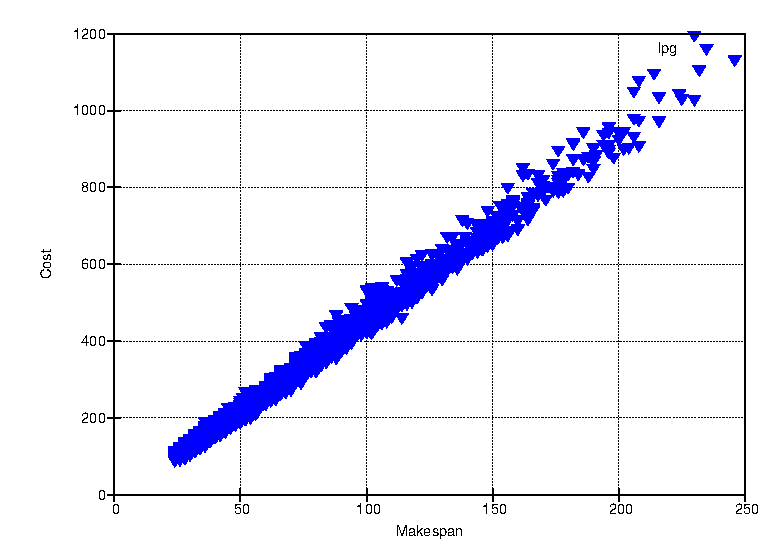
\includegraphics[bb=50 50 410 302,scale=0.75]{../plot_archive/foortilePfile0_Add_lpg_pareto.eps}}\\
 \subfloat[floortile3]{\includegraphics[bb=50 50 410 302,scale=0.75]{../plot_archive/foortilePfile3_Add_lpg_pareto.eps}}
 \subfloat[floortile4]{\includegraphics[bb=50 50 410 302,scale=0.75]{../plot_archive/foortilePfile4_Add_lpg_pareto.eps} }\\
 \subfloat[openstacks-p01]{\includegraphics[bb=50 50 410 302,scale=0.75]{../plot_archive/openstacks_p01_Add_lpg_pareto.eps}}
   \caption{LPG}
\end{center}
  \end{figure*}

 \newpage
 

  \begin{figure*}[h!]
 \begin{center}
 \subfloat[ openstacks-p01]{\includegraphics[bb=50 50 410 302,scale=0.75]{../plot_archive/openstacks_p01_Add_p_pareto-graphic.eps}}
 % elevator_p01-p04_Add_lpg_pareto.eps: 0x0 pixel, 300dpi, 0.00x0.00 cm, bb=50 50 410 302
 \subfloat[floortile0]{\includegraphics[bb=50 50 410 302,scale=0.75]{../plot_archive/floortilePfile0_Add_p_pareto-graphic.eps}}\\
 \subfloat[floortile3]{\includegraphics[bb=50 50 410 302,scale=0.75]{../plot_archive/floortilePfile3_Add_p_pareto-graphic.eps}}
 \subfloat[floortile4]{\includegraphics[bb=50 50 410 302,scale=0.75]{../plot_archive/floortilePfile4_Add_p_pareto-graphic.eps} }\\
 \subfloat[elevator-p01-p04]{\includegraphics[bb=50 50 410 302,scale=0.75]{../plot_archive/elevators_p01-p04_Add_p_pareto-graphic.eps}}
    \caption{DAE$_yahsp$ Vs LPG}
\end{center}


  \end{figure*}
 
 
 
 
  \begin{figure*}[h!]
 \begin{center}
  \subfloat[floortile0]{\includegraphics[bb=50 50 410 302,scale=0.75]{../plot_archive/floortilePfile0_Add_p_pareto-bounds.eps}}\\
 \subfloat[floortile3]{\includegraphics[bb=50 50 410 302,scale=0.75]{../plot_archive/floortilePfile3_Add_p_pareto-bounds.eps}}
 \subfloat[floortile4]{\includegraphics[bb=50 50 410 302,scale=0.75]{../plot_archive/floortilePfile4_Add_p_pareto-bounds.eps} }\\
    \caption{DAE$_yahsp$ Vs LPG}
\end{center}


  \end{figure*}
  
 
 \section{Multi-Evals}
  \begin{figure*}[h!]
 \begin{center}
   \subfloat[floortile0]{\includegraphics[bb=50 50 410 302,scale=0.75]{../plot_archive/floortile0_dae_eval_pareto.eps}}
 \subfloat[floortile3]{\includegraphics[bb=50 50 410 302,scale=0.75]{../plot_archive/floortile3_dae_eval_pareto.eps}}\\
 \subfloat[floortile4]{\includegraphics[bb=50 50 410 302,scale=0.75]{../plot_archive/floortile4_dae_eval_pareto.eps}}
  \subfloat[openstacksp01]{\includegraphics[bb=50 50 410 302,scale=0.75]{../plot_archive/openstacksp01_dae_eval_pareto.eps}}\\
    \subfloat[openstacksp05]{\includegraphics[bb=50 50 410 302,scale=0.75]{../plot_archive/openstacksp05_dae_eval_pareto.eps}}
      \subfloat[openstacksp10]{\includegraphics[bb=50 50 410 302,scale=0.75]{../plot_archive/openstacksp10_dae_eval_pareto.eps}}\\
       
        
        \end{center}
    \caption{Multi-Evals}

  \end{figure*}
  
  \begin{figure*}[h!]
 \begin{center}
 
 \subfloat[openstacksp15]{\includegraphics[bb=50 50 410 302,scale=0.75]{../plot_archive/openstacksp15_dae_eval_pareto.eps}}
  \subfloat[openstacksp20]{\includegraphics[bb=50 50 410 302,scale=0.75]{../plot_archive/openstacksp20_dae_eval_pareto.eps}}\\
        
  \end{center}
    \end{figure*}
    
    
    
    
    
    
    
    
  
%  \begin{figure*}[h!]
%  \centering
%    \subfloat[zenoTravel-zfile1] {\includegraphics[bb=50 50 410 302,scale=0.75]{../plot_archive/zenoTravel_zfile1__Add_ibeahyper_pareto.eps}}
%     \subfloat[zenoTravel-zfile10] {\includegraphics[bb=50 50 410 302,scale=0.75]{../plot_archive/zenoTravel_zfile10_Add_ibeahyper_pareto.eps}}
%  % zenoTravel_zfile1__Add_ibeahyper_pareto.eps: 0x0 pixel, 300dpi, 0.00x0.00 cm, bb=50 50 410 302
%    \caption{zenoTravel}
%  \end{figure*}
%  
%  \begin{figure*}[h!]
%  \centering
%   \subfloat [zeno3e-LPG] {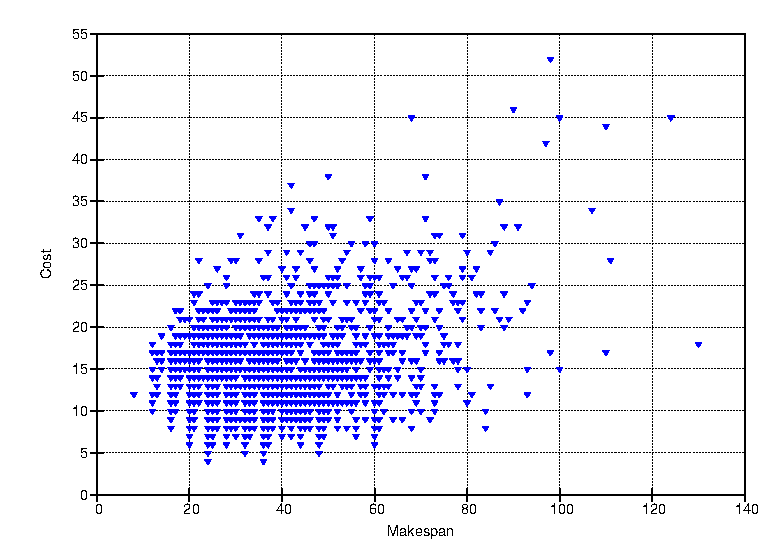
\includegraphics[bb=50 50 410 302,scale=0.75]{../plot_archive/zeno3elg_Add_daelpg_pareto.eps}}
%  % zeno3elg_Add_daelpg_pareto.eps: 0x0 pixel, 300dpi, 0.00x0.00 cm, bb=50 50 410 302
%   \caption{LPG}
%  \end{figure*}


\end{document}